% Options for packages loaded elsewhere
\PassOptionsToPackage{unicode}{hyperref}
\PassOptionsToPackage{hyphens}{url}
%
\documentclass[
]{book}
\usepackage{amsmath,amssymb}
\usepackage{lmodern}
\usepackage{ifxetex,ifluatex}
\ifnum 0\ifxetex 1\fi\ifluatex 1\fi=0 % if pdftex
  \usepackage[T1]{fontenc}
  \usepackage[utf8]{inputenc}
  \usepackage{textcomp} % provide euro and other symbols
\else % if luatex or xetex
  \usepackage{unicode-math}
  \defaultfontfeatures{Scale=MatchLowercase}
  \defaultfontfeatures[\rmfamily]{Ligatures=TeX,Scale=1}
\fi
% Use upquote if available, for straight quotes in verbatim environments
\IfFileExists{upquote.sty}{\usepackage{upquote}}{}
\IfFileExists{microtype.sty}{% use microtype if available
  \usepackage[]{microtype}
  \UseMicrotypeSet[protrusion]{basicmath} % disable protrusion for tt fonts
}{}
\makeatletter
\@ifundefined{KOMAClassName}{% if non-KOMA class
  \IfFileExists{parskip.sty}{%
    \usepackage{parskip}
  }{% else
    \setlength{\parindent}{0pt}
    \setlength{\parskip}{6pt plus 2pt minus 1pt}}
}{% if KOMA class
  \KOMAoptions{parskip=half}}
\makeatother
\usepackage{xcolor}
\IfFileExists{xurl.sty}{\usepackage{xurl}}{} % add URL line breaks if available
\IfFileExists{bookmark.sty}{\usepackage{bookmark}}{\usepackage{hyperref}}
\hypersetup{
  pdftitle={Linear Algebra: An Intuitionist Approach},
  pdfauthor={Matt Pettis},
  hidelinks,
  pdfcreator={LaTeX via pandoc}}
\urlstyle{same} % disable monospaced font for URLs
\usepackage{longtable,booktabs,array}
\usepackage{calc} % for calculating minipage widths
% Correct order of tables after \paragraph or \subparagraph
\usepackage{etoolbox}
\makeatletter
\patchcmd\longtable{\par}{\if@noskipsec\mbox{}\fi\par}{}{}
\makeatother
% Allow footnotes in longtable head/foot
\IfFileExists{footnotehyper.sty}{\usepackage{footnotehyper}}{\usepackage{footnote}}
\makesavenoteenv{longtable}
\usepackage{graphicx}
\makeatletter
\def\maxwidth{\ifdim\Gin@nat@width>\linewidth\linewidth\else\Gin@nat@width\fi}
\def\maxheight{\ifdim\Gin@nat@height>\textheight\textheight\else\Gin@nat@height\fi}
\makeatother
% Scale images if necessary, so that they will not overflow the page
% margins by default, and it is still possible to overwrite the defaults
% using explicit options in \includegraphics[width, height, ...]{}
\setkeys{Gin}{width=\maxwidth,height=\maxheight,keepaspectratio}
% Set default figure placement to htbp
\makeatletter
\def\fps@figure{htbp}
\makeatother
\setlength{\emergencystretch}{3em} % prevent overfull lines
\providecommand{\tightlist}{%
  \setlength{\itemsep}{0pt}\setlength{\parskip}{0pt}}
\setcounter{secnumdepth}{5}
\usepackage{booktabs}
\usepackage{braket}
\ifluatex
  \usepackage{selnolig}  % disable illegal ligatures
\fi
\usepackage[]{natbib}
\bibliographystyle{plainnat}

\title{Linear Algebra: An Intuitionist Approach}
\author{Matt Pettis}
\date{2021-11-05}

\begin{document}
\maketitle

{
\setcounter{tocdepth}{1}
\tableofcontents
}
\hypertarget{preface}{%
\chapter{Preface}\label{preface}}

\begin{quote}
And you may ask yourself, ``What is that beautiful house?''

And you may ask yourself, ``Where does that highway go to?''

And you may ask yourself, ``Am I right? Am I wrong?''

And you may say to yourself, ``My God! What have I done?''

-- Talking Heads, ``Once in a Lifetime''
\end{quote}

\begin{quote}
What one fool can do, another can.

-- Ancient Simian Proverb

-- Sylvanus Thompson, ``Calculus Made Easy''
\end{quote}

\begin{quote}
``Everything is the way it is because it got that way.''

-- D'Arcy Wentworth Thompson
\end{quote}

I'd like to say I'm writing this ``for the democratization of science and math,'' but really, for my kids and their friends so that they don't get snookered into thinking this stuff is beyond them and therefore not for them. It is for you. It is everybody's birthright.

One of the best things about science, but one I've found least talked about in the classes that I took in high school and college, is the part that explains ``why do we think things work this way?'' Why do we believe things are made up of atoms? Why did people believe that without the ability to \emph{see} atoms? What is it about the technology we've built that confirms that things are made of atoms? We believe things like this because we concocted hypotheses and made experimental tests that ruthlessly and cumulatively. We make assumptions that are verifiably true, and then we reach a little further with logic and some more subtle observations, and extend the things we get to conclude, and what we have to throw away. That is a powerful process.

Somewhere along the way, math got divorced from that process. It wasn't helped by great mathematicians like Carl Gauss who called Number Theory ``the Queen of Mathematics'' mostly because it didn't have much in the way of application, and that was a good thing. Or the eminent mathematician G. H. Hardy, who said,

\begin{quote}
``I have never done anything''useful``. No discovery of mine has made, or is likely to make, directly or indirectly, for good or ill, the least difference to the amenity of the world.''
\end{quote}

The perspective was, and often is, that math is a thing more akin to art, like poetry, and though it is sometimes useful, its main value is in that it is beautiful and fun. Ironically, his favorite subject, number theory, is the foundation of our ability to transmit secrets safely on the internet, and does, in fact, probably cause more good and ill than he was comfortable with.

The downside of such a perspective is that it makes it seem like learning the discipline of mathematics is inscrutable. When you encounter mathematical definitions, such as, ``What makes a thing a vector space?'', or ``What makes a thing a group?'', or ``What makes a set measureable?'', what you read are a bunch of seemingly awkward little statements that seem either indecipherable, or unknowable, or so stupidly dead-simple as to make you wonder why one would even need to say such a thing. For instance, when we get to the definition of a vector space, you'll see this as a defining characteristic that your, uh, we'll call a thingy for now, needs to have to be called a vector space:

\[ (\vec{x} + \vec{y}) + \vec{z} = \vec{x} + (\vec{y} + \vec{z}) \]

For those familiar with how numbers work, this seems like something Captain Obvious would say about math. It could also make you wonder ``what's the point of saying such a thing?''

These definitions don't come in an inspiration, like Athena springing fully formed from the forehead of Zeus. When you study the history of mathematics, you'll see that when trying to come up with descriptions like this, mathematicians will often argue, and even disagree violently. You'll often see different characterizations like this depending on where you look, because originators disagreed on what was \emph{fundamental} about what was going on. For systems to be compatible, though, the fundamental assumptions of one camp need to be at least derivable from the other, and vice versa.

This monograph is intended give you the motivations of why linear algebra is the way it is. It will address:

\begin{itemize}
\tightlist
\item
  Where do those rules about a vector space come from?
\item
  What's the big deal about linear independence?
\item
  What would make you come up with an idea like an inner product?
\item
  What's helpful about orthogonality?
\item
  Eigenvectors: how do they even work?
\end{itemize}

I'll approach this as science would ideally approach this. What do we observe? What sort of simplifications can we make to help us understand what is going on? What sort of models help us understand the important parts?

\hypertarget{well-how-did-i-get-here}{%
\chapter{Well, How Did I Get Here?}\label{well-how-did-i-get-here}}

\begin{quote}
It takes a very unusual mind to undertake the analysis of the obvious.

Alfred North Whitehead
\end{quote}

At this point, if you are reading this as opposed to an intro to linear algebra book, I assume the one thing you have is a good familiarity with are the vector spaces of \(\mathbb{R}^2\) and \(\mathbb{R}^3\). These are the vector spaces used extensively in physics and engineering to model things like position, velocity, and forces.

You know that you can add two vectors by putting the tail of one vector at the head of the other and connecting the base of one to the tip of the other vector.

\begin{figure}

{\centering 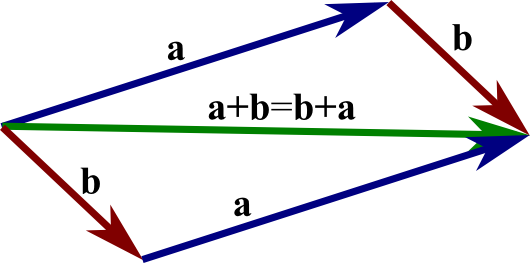
\includegraphics[width=0.75\linewidth,height=0.75\textheight]{images/vector_parallelogram_law} 

}

\caption{Parallelogram Law of Addition}\label{fig:unnamed-chunk-1}
\end{figure}

And we know how to stretch, shrink, and flip a vector, which we do by multiplying a vector by a real number. If you multiply a vector by \(1/2\), the length of the vector shrinks to one-half its original length (but the direction doesn't change). If you multiply a vector by \(3 \sqrt{2}\) the magnitude of the result is stretched by that amount.

\begin{figure}

{\centering 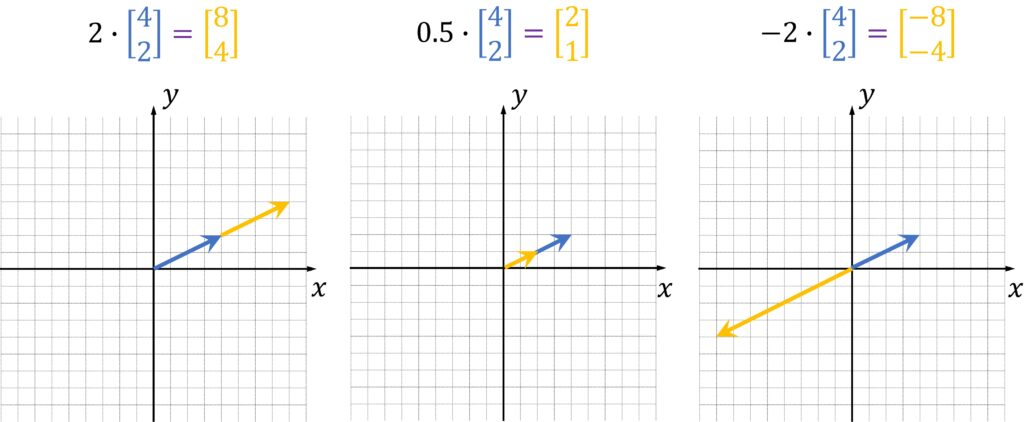
\includegraphics[width=1\linewidth,height=1\textheight]{images/Vector-scaling} 

}

\caption{Vector Scaling}\label{fig:unnamed-chunk-2}
\end{figure}

These are the prototypical vector spaces, one I'd argue 99 times out of 100 people imagine if they know what a vector space is already. And if this is the only space you have to deal with, this intuition is pretty much all you need. It will take you far. But if you study quantum state space vectors, with their complex entries, and the notion of \(\mathbb{R}^n\) vector spaces can help some of your intuition, and for other parts, you are totally at sea as to how the hell you are supposed to interpret things.

So it may help to go back to \(\mathbb{R}^n\) and do some careful syntax-to-interpretation explanations. And take some of the things we take for granted as obvious and cast them in new, abstract lights.

Before we get to the vector space axioms, let's review our intuitions a bit more about \(\mathbb{R}^n\) vector spaces.

\hypertarget{intuition-about-mathbbrn}{%
\section{\texorpdfstring{Intuition about \(\mathbb{R}^n\)}{Intuition about \textbackslash mathbb\{R\}\^{}n}}\label{intuition-about-mathbbrn}}

We already discussed how addition and scalar multiplication are performed. But we should note the choices we made to do what seems so natural to us.

First, addition. We did it using the parallelogram law. How come we didn't choose to make the resulting vector have a length equal to the sum of the length of the two starting vectors? You can see from the picture the length of our resulting vector is usually shorter, but never longer, than the length of the two vectors you are adding. You should counter, ``well, that's because things like forces don't work that way. If I have two equal and opposite forces acting on an object, I want the result to be no net force. If the magnitudes were added, which direction would the result point? Doesn't make sense, so we can't use that because it doesn't model the situation.''

Good answer, reader!

We want our model to reflect what is going on. So that sort of addition is out. It turns out head-to-tail addition does model things like forces. What is also intuitive is that for any arrow, or force, or velocity, you can ``counteract'' it with another arrow/force/velocity. You could not do this if the magnitues themselves always add. You can never add two positive things to get a net zero, which would represent two things counteracting each other.

Second, just what do we mean by multiplying a vector by a scalar? That's a little trickier. We know what we mean: we shrink and grow the vector, in the same direction, by the scalar's sign and magnitude. As above, multiplying a vector by \(1/2\) shrinks its length to \(1/2\) the original length, but the direction stays the same.

But if you are an engineer or scientist, your unit-analysis Spidey-sense should start to tingle\ldots{} if scalars and vectors are different things, and I multiply them, whatever happens, I shouldn't get a vector out, like we are seeing.

A dirty little detail is usually glossed over. Because it is short-circuiting to your intuition about stretching or shrinking, people don't talk about what \(\alpha \vec{x}\) is. Your brain probably assumes it is a multiplication, and what the scalar is multiplying is the ``magnitude'' property of the vector. You can think about it that way for \(\mathbb{R}^n\) vectors. But that's not really a scalar-vector multiplication. What it really is is the scalar acting as a function that maps a vector to another vector. Like so:

\[ f_{\alpha} : V \to V , \alpha \in \mathbb{R} \]
So, \(\alpha \vec{x}\) is really shorthand for \(f_{\alpha}(\vec{x})\).

For \(\mathbb{R}^n\), that function is the function that stretches or shrinks the magnitude of the vector by \(\alpha\). Again, this may seem like nit-picky pedantry, but we have to start leveraging this fact in the near future to keep some other things clear\ldots{}

\hypertarget{the-axioms}{%
\section{The Axioms}\label{the-axioms}}

So if vector spaces were just stretching and head-to-tail vector additions, mathematicians probably wouldn't make the seemingly awkward definition that are always presented in the first three pages of any textbook:

From Wikipedia:

\begin{figure}

{\centering 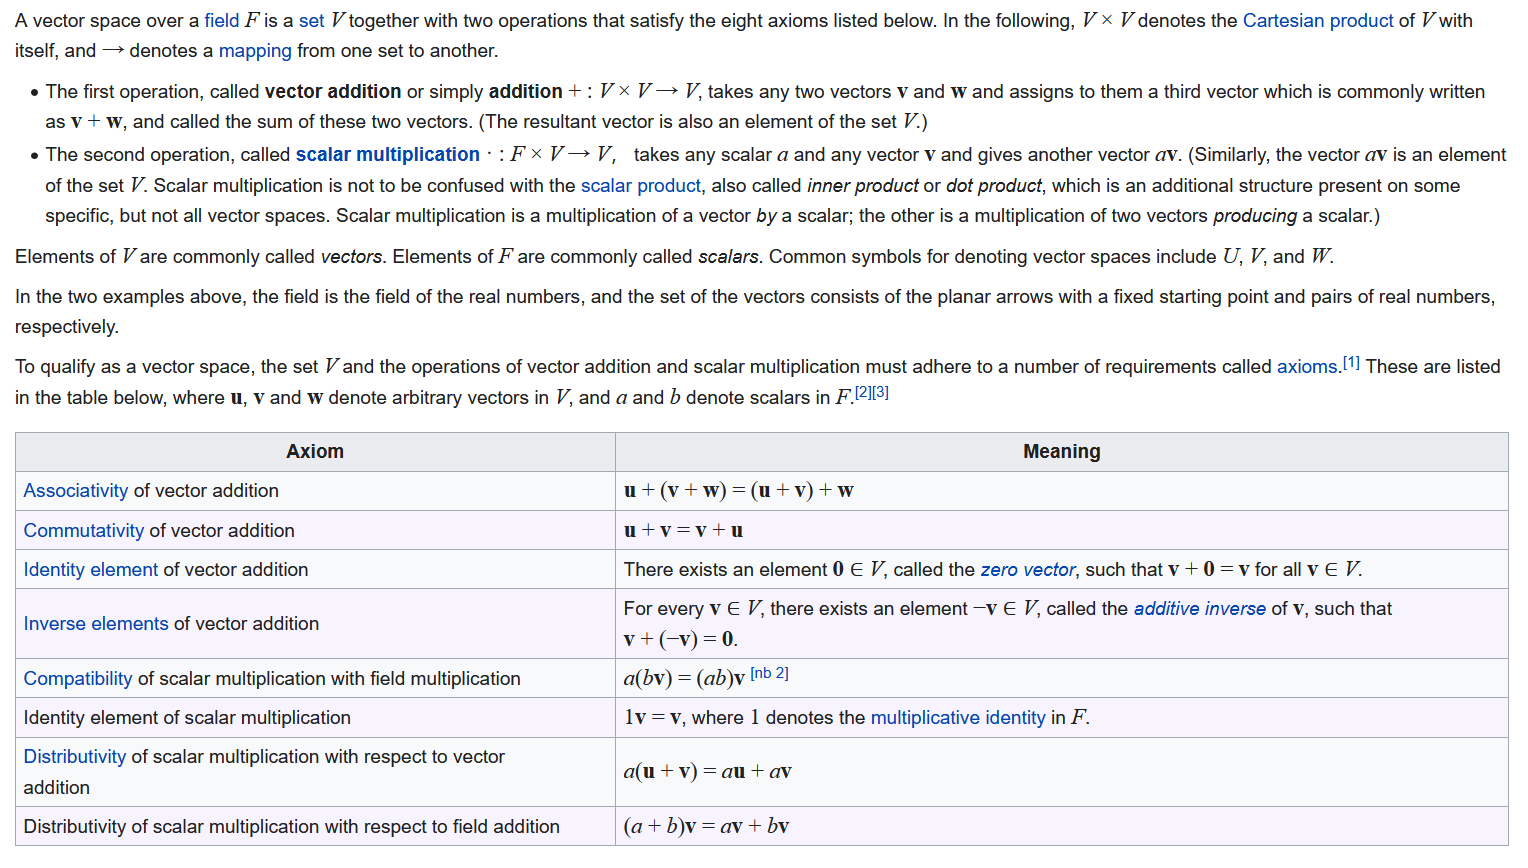
\includegraphics[width=1\linewidth,height=1\textheight]{images/vector-space-axioms-wikipedia_2} 

}

\caption{[Record scratch]  Yep, that's me, Vector Space, spewing a lot of incomprehensible stuff.  But I wasn't always like this.  Let me tell you a story...}\label{fig:unnamed-chunk-3}
\end{figure}

It is a bad way to start, because you really have no frame of reference for what any of the terms mean. It is frustrating and made me angry \textbf{We shouldn't really start here.}

This reminds me of the joke about a cab driver driving around the Seattle area in a fog, and he asks a guy coming out of a building if he can tell the cabbie where he is. The guy looks at him and says, ``You're in a cab,'' and walks on. The cabbie says ``Perfect, I know where I am.'' The fare asks him how he can figure out anything from what the guy outside said, and the cabbie say, ``Well, he told me something that was completely true and completely useless. So this must be the Microsoft building.''

There's so many questions that should be triggered. Like:

\begin{itemize}
\tightlist
\item
  Why so many simple axioms?
\item
  What are vectors, really?
\item
  What is a field, really?
\item
  What does it mean to add vectors?
\item
  What does it mean to multiply a vector by a scalar?
\item
  How do I know what other vector \(a \cdot \vec{u}\) becomes?
\item
  It looks like the scalar field talks about how \emph{scalar addition} and \emph{scalar multiplication} works. But vectors only talk about \emph{vector addition}. What's up with that?
\end{itemize}

With \(\mathbb{R}^n\), we can look over the axioms and confirm that yep, they meet the axioms, because we have a strong intuition about how addtion of vectors work, how scalars stretch the vectors, and how the addition and multiplication of scalar (read: real) numbers work.

We can boil these axioms down as follows:

\begin{itemize}
\tightlist
\item
  It won't matter what order you do your operations in, you are guaranteed to get the same answer. All of the axioms that deal with associativity, commutativity, compatibility, and distributivity are telling us.
\item
  Your vector space has an element that acts as a \(\vec{0}\) element, and every vector has an opposite that, when you add them together, gives you \(\vec{0}\).
\item
  Your scalar field, which has a \(\vec{1}\) in it, when combined with a vector, won't change that vector.
\end{itemize}

But that doesn't answer why we say what we want in a vector space that way. Even more, we don't have a good idea of what other structures my meet these axioms and be a vector space. Or how to interpret that.

\hypertarget{why-are-the-axioms-this-way}{%
\section{Why are the axioms this way?}\label{why-are-the-axioms-this-way}}

In elementary school, you learned your 1-digit by 1-digit times tables by rote. And then you learned how you could leverage that to multiply numbers bigger than 1-digit together by using the 1-digit table entries, putting the results in certain columns, learning how to carry, write down partial sums, and add them together. You need only know the 1-digit times tables and a procedure with adjusted addition to handle the multiplication of any two numbers of any length.

\emph{That} reduction to a set of memorized computations and easy rules to combine the results to get us any arbitrary computation is what we are striving for in vector spaces. We don't want to have to memorize the sum of every two-vector combination in the space, because by my last count, I'm pretty sure there are more than 57 vectors in \(\mathbb{R}^2\) alone. What we want is a nice way to get a fixed set of facts we have to know about, and find simple procedures to compute the facts only as we need them.

So here's the game plan, to try and tackle complex things like \(\mathbb{R}^n\) and other things that will qualify as vector spaces. We are going to reference some topics that will be familiar to you if you've dealt with linear algebras before, but haven't talked about yet here:

\begin{longtable}[]{@{}
  >{\raggedright\arraybackslash}p{(\columnwidth - 2\tabcolsep) * \real{0.53}}
  >{\raggedright\arraybackslash}p{(\columnwidth - 2\tabcolsep) * \real{0.47}}@{}}
\toprule
Task & Vector space concept \\
\midrule
\endhead
Get a fixed number of facts (vectors \(\vec{x}_{i}\)) we need to deal with, like the times table. & Pick linearly independent vectors \(\vec{x}_{i}\). \\
Figure out how to express them as simple combinations of known facts & Linear combinations with scalars: \(\vec{x} = \alpha_{1} \vec{x}_{1} + \alpha_{1} \vec{x}_{1} + ... + \alpha_{n} \vec{x}_{n}\). A minimal set of linearly independent vectors that can do this is called a \emph{basis}. \\
Discover that for vector spaces (finite ones), any set of vectors that work to do this \emph{always} has the same number of vectors & This is the dimensionality \(N\) of the space. \\
Figure out how to calculate \(\alpha_{i}\) for a given set of vectors. & To do this, we'll have to create the concept of the \emph{inner product}. \\
Find out that lots of choices of \(\vec{x}_{i}\) will work to express any vector, but \emph{certain} ones are easier to compute the \(\alpha_{i}\)'s for. & These will vectors that are orthogonal and of a certain size (magnitude = 1). The word that captures both of these concepts is \emph{orthonormal}. There are still lots of orthonormal sets. \\
Figure out how to take an arbirary linear independent set and construct an equivalent orthonormal set out of them, because they are easier to deal with. & This is the Gram-Schmidt theorem. \\
\bottomrule
\end{longtable}

This will be enough for now. Once we get into functions \emph{between} vector spaces, and pick out the special functions (the \emph{linear} transforms), we'll talk about what \emph{eigenvectors} and \emph{eigenvalues} are. But not yet.

The insight here is that for a given vector space, rather than work with the raw vectors themselves, it is easier to break them down into computations on known vectors (the basis), and do scalar multiplication (really, mappings that work like the underlying arithmetic on the scalars) on those basis vectors. This is because the operations on the scalar field, and the way they map (or stretch) the basis vectors is ultimately an easier accounting scheme. So we go through all of this work to find linear independent sets, basis, orthonormal bases, etc., so that we can use the inner product to easily get scalar coefficients and go on our merry way doing calculations on the vector space elements themselves.

\ldots{}

You could think about this as follows: all you have are the vectors, and you are given a really big set of rules that tells you what vector you get when you add any two vectors. You just have to find that rule in the set. It would be like memorizing your times tables way way far beyond your 1-digit by 1-digit table you have in elementary school. Some savants do this to perform faster computations -- they may memorize all 2-digit by 2-digit products, and that can significantly speed up their already fast computations. Some even have some key 3-digit by 3-digit products memorized.

If you think about it, in \(\mathbb{R}^n\), that scalar relationship is a pattern you notice about how the vectors adhere to. But it isn't necessary -- you could just memorize what resulting vector you get when you add any two vectors together.

Here's one of the guiding intuitions about vector spaces. Vector spaces are huge. Like, I'm pretty sure there are more than 57 vectors in \(\mathbb{R}^2\) alone.

The point here is this: we have a good intuitive idea of how vectors behave in \(\mathbb{R}\) spaces. As we stated above, we can just follow our noses: scalars can be added and multiplied, vectors can be added, and we can put them together in ways such that if we construct a vector \(\vec{x} = \alpha_{1} \vec{x_{1}} + \alpha_{2} \vec{x_{2}}\), we can figure out exactly what vector \(\vec{x}\) we must have.

But we don't \emph{have} to rely on that geometry of arrows in general, and how they stretch and add with the parralelogram rule. We don't have to have any idea what the elements of the vector space really look like (as in, they don't have to be arrows in \(\mathbb{R}\) space). They just have to be objects that have a vector \(+\) structure, and you can define some maps on those objects, which you can \emph{label} with scalars (from \(\mathbb{R}\) or \(\mathbb{C}\), as we'll see), and they just have to obey the axioms. We will need to lift off from this \(\mathbb{R}\) prototype of vector spaces for some of the vector spaces we will use in quantum theory. At first, you will want to use your intuition about \(\mathbb{R}\) to reason about these more abstract vector spaces (the quantum ``state space''), but it won't \emph{quite} work, and you'll need this more sophisticated abstraction.

In the next chapter, we'll take some quantum phenomenon, and figure out how we pick linear algebra to model our phenomenon, and what tools from its toolbox we will need. And illuminate a little more how linear algebra hangs together.

\hypertarget{how-do-i-work-this}{%
\chapter{How do I work this?}\label{how-do-i-work-this}}

My uncle tells the story of how they help transition mechanical engineers fresh out of school to working in industry. A senior engineer tasks them with a simple task: a near complete machine needs a piece -- it is missing a cog. The tell the new engineer to get them one. The new engineer studies the plans, designs the cog, painstakingly laying out the CAD designs for it, and comes back to the senior engineer after a week with his work to review how to machine that part, and how much it will cost. The senior engineer looks it over, says it is the right piece, and pulls out a catalog, and shows him how much it will cost to buy, usually at a fraction of the cost. The lesson they learn: don't create from scratch stuff you can buy cheaply from a catalog.

We might think of physics and mathematics having a similar relationship. Often, as you painstakingly observe a physical system, you figure out what are the important bits you need to capture with a model, and how those bits behave in the system. Then, you go shopping to your local math department, describing what you are doing, and hope that a mathematician can recommend a system they've already investigated that you can map your problem into, and take advantage of the notions, the notations, and theorems about the system behavior that they've already come up with.

So, let's proceed by looking at a simple spin-\(1/2\) system, of electrons that can have either a spin up or down measurement, depending on how the spin-detector is oriented. Many newer books start their quantum discussion this way, and two I can recommend that do this are \emph{Quantum Mechanics: The Theoretical Minimum} by Len Susskind and \emph{Quantum Mechanics: A Paradigms Approach} by David McIntyre. I won't repeat their treatment here, and will assume you know the basics of measuring spins in those systems. I will talk about how you start to pick your mathematics from the catalog to model this phenomenon.

\hypertarget{lay-of-the-land}{%
\section{Lay of the Land}\label{lay-of-the-land}}

Here is a picture that captures some of the important information about a quantum experiment we run:

\begin{figure}

{\centering 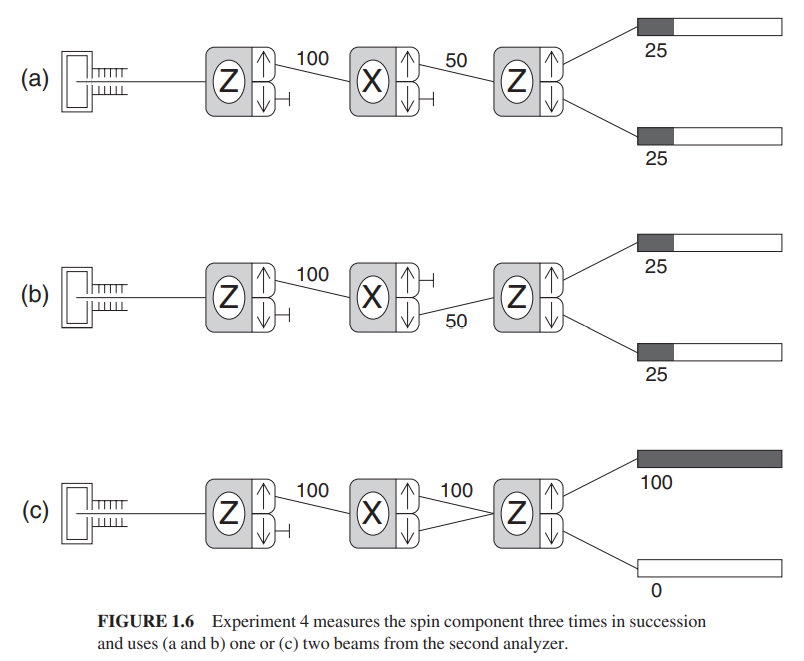
\includegraphics[width=0.75\linewidth,height=0.75\textheight]{images/McIntyre_two-spin-experiment} 

}

\caption{Two-spin experiment, McIntire}\label{fig:unnamed-chunk-4}
\end{figure}

Some notes on the picture:

\begin{itemize}
\tightlist
\item
  The apparatus on the left emits electrons, which have a spin we want to measure.
\item
  The detectors are labeled with a `Z' or `X' to tell you which direction in space we are orienting the detector. We pick the directions arbitrarily, but `Z' and `X' are orthogonal directions.
\item
  The arrows on the detectors indicate which spin orientation an electron comes out of. If it is measured with a spin up, relative to the how the detector is oriented, it exits from the top port, with the up arrow. If down, it exits from the lower port.
\item
  The labels \texttt{\textbar{}+\textgreater{}} and \texttt{\textbar{}-\textgreater{}} are also labels for the spins. The indicate absolute directions of the spin (spin up or down in the Z direction), rather than the up and down arrows on the port, that indicate if the spin is up or down \emph{relative to the how the port is oriented}, in the `Z' or `X' direction.
\item
  The labels \texttt{\textbar{}+\textgreater{}}\_x and \texttt{\textbar{}-\textgreater{}}\_x represent the absolute spin up/down orientations, but for the X direction. Again, the detector can be reoriented, but if the electron has one of these labels, it is independent of how the detector is oriented.
\item
  The numbers and shaded bars represent a percentage of electrons that end up in that bucket or state over a large number of electrons entering the system. Like a histogram.
\end{itemize}

Here are some things you, the experimenter, observe about the system:

\begin{itemize}
\tightlist
\item
  In (a), if you measure the Z spin, then the X spin, then the second time you measure the Z spin, it will be 50-50 up/down.
\item
  In (b), it just tells you that the same thing happens, no matter if the secon measurement for X is up or down, like in experiment (a).
\item
  In (c), somthing really weird happens: If you put the X spin detector in the middle, but carefully recombine both beams, as if you didn't measure the X spin, then the Z spin will be as if you didn't measure X spin at all, and stays in the spin state you measured it in in the first detector.
\end{itemize}

That can stand as the first of many weirdnesses you encounter in quantum. As McIntyre says: going from (a) or (b) to (c), it's as if you are in a half-lit room, throw open a window shade, and the whole room goes dark. In a classical model, (c) would still have a 50-50 split of spin measurements, but that doesn't happen in the quantum world.

\hypertarget{what-things-do-we-need-to-model-this}{%
\section{What things do we need to model this?}\label{what-things-do-we-need-to-model-this}}

So, we make the following observations.

\begin{itemize}
\tightlist
\item
  If we measure a spin as up in the Z direction, and keep measuring the spin with detectors all pointed along the same Z axis, we will always get the same spin up measurement. That is true as long as we don't orient the detector in a different direction.
\item
  Focusing on Z measurements, we have two states: spin up (\texttt{\textbar{}+\textgreater{}}) and spin down (\texttt{\textbar{}-\textgreater{}}). We get that with the detector registering a +1 or -1.
\item
  If we measure a Z spin with a detector, and it registers a +1, we call it spin up, and take a second, identical detector, and flip it upside, it will register a -1. This scenario is not pictured.
\item
  If we take a Z detector and measure a spin up electron, and then take a second detector, and start to slightly tilt the detector away from a straight Z orientation, we still only measure +1 and -1 readings. For a slight tilt, almost all electrons will measure spin up, and a few spin down. As it rotates to be perpendicular to the Z direction, electrons measure +1 and -1 with a 50\% probability. As we get closer to the tilt making the detector upside down, then most of the electrons will measure -1, until it is exactly upside down, and the detetcor will consistently measure -1.
\end{itemize}

This is kind of weird. Note that if this were a classical spin, you would expect that if you measured a spin of +1, and tilted the detector a little bit, you would measure a value a little less than +1. But quantum doesn't work that way. Instead of reducing the spin a little bit, what happens is that the probability of a +1 starts to decrease as you tilt the detector. The \emph{average} of multiple measurements approaches the value of what you would expect a single measured spin to decrease by (if it were classical).

So, whatever math we come up, it can't be the same classical math that gives a single spin measurement decreasing continuously from +1. It has to be something that accounts for:

\begin{itemize}
\tightlist
\item
  A spin will always either be +1 or -1
\item
  The \emph{probability} of detecting +1 and -1 change as you tilt the detector.
\end{itemize}

So we go talk to the math department\ldots{}

  \bibliography{book.bib,packages.bib}

\end{document}
